\section{Introducci\'on te\'orica}

El problema de Demosaicing consta de poder construir una imagen con información de los 3 canales en cada uno de sus pixel en base a una que sólo tiene definidos los valores de un sólo canal para cada celda. Este desafío es muy común en las camáras de fotos digitales ya que en realidad cada fotosensor detecta un sólo color, por lo cual a la imagen capturada hay que aplicarle algún procedimiento lógico para que el usuario final pueda verla efectivamente con todos los colores.

Particularmente estaremos analizando 4 algoritmos distintos que intentan solucionar esto. Ellos son: Vecinos, Bilineal, Direccional y High Quality. Todos estos deben aplicarse sobre imágenes en formato Bayer array, es decir, imágenes que en cada pixel tienen información sólo de un canal (Verde, Rojo o Azul) y estos además tienen una distribución especial (en la que por ejemplo el verde predomina en cantidad ya que es el color que mejor recepción tiene en el ojo humano).

Para nuestras pruebas lo que haremos es tomar imágenes con todos sus canales completos en todos lo pixeles y pasarlas al formato Bayer array. Como en lo que queremos hacer foco en este trabajo es la calidad de estos procedimientos y sus resultados, no nos interesa que la imagen Bayer haya sido tomada realmente por una cámara, es más, nos sirve más tener una imagen full color y transformala ya que así podemos comparar nuestros resultados contra la original.

Por esto es que desarrollamos una función muy simple que realiza esta transformación. Básicamente lo que hace es: 
\begin{itemize}
\item Celdas en columnas y filas pares, deja sólo el canal azul
\item Celdas en columnas y filas impares, deja sólo el canal rojo
\item En todas las otras dejamos sólo el canal verde
\end{itemize}   


\begin{figure}[h]
       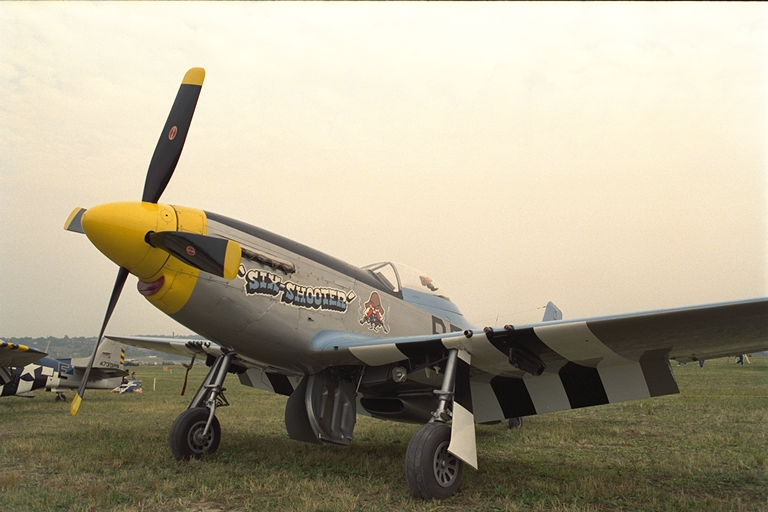
\includegraphics[width=0.5\textwidth]{imagenes/img9.png}
           \hfill
        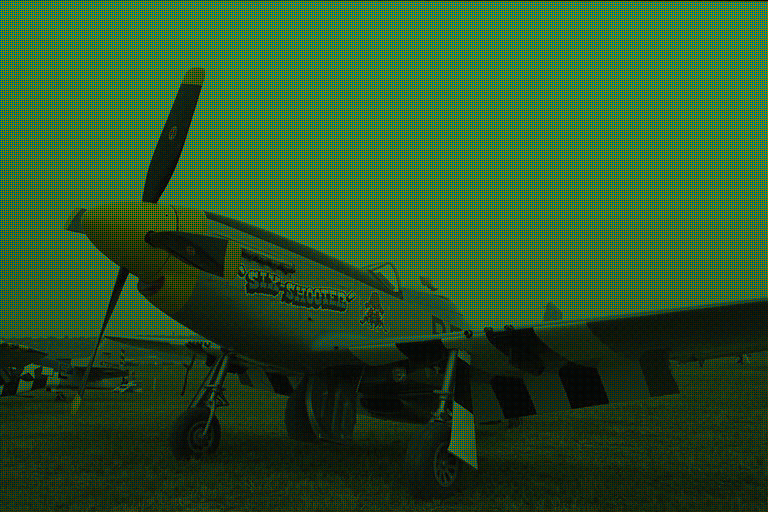
\includegraphics[width=0.5\textwidth]{imagenes/img9_bayer.png}   
        Imagen original y bayerizada
\end{figure}

\subsection{Artifacts}